%==========================================================
%  Spectrum-SLM — Clean Light Beamer Presentation
%==========================================================
\documentclass[aspectratio=169, 10pt]{beamer}

\usetheme{Madrid}
\usecolortheme{whale}
\usefonttheme{professionalfonts}
\setbeamertemplate{navigation symbols}{}
\setbeamertemplate{headline}{}
\setbeamersize{text margin left=6mm, text margin right=6mm}

% ── Packages ─────────────────────────────────────────────
\usepackage[utf8]{inputenc}
\usepackage[T1]{fontenc}
\usepackage{lmodern}
\usepackage{amsmath,amssymb}
\usepackage{booktabs}
\usepackage{array}
\usepackage{graphicx}
\usepackage{tikz}
\usetikzlibrary{shapes.geometric, arrows.meta, positioning, calc}
\usepackage{pgfplots}
\pgfplotsset{compat=1.18}
\usepackage{listings}
\usepackage{pifont}
\usepackage{xcolor}
\usepackage{colortbl}

% ── Colors ───────────────────────────────────────────────
\definecolor{navy}{HTML}{1B2A4A}
\definecolor{royalblue}{HTML}{2E5090}
\definecolor{teal}{HTML}{0E8C7F}
\definecolor{coral}{HTML}{E05555}
\definecolor{amber}{HTML}{D4920B}
\definecolor{lightbg}{HTML}{F4F6FA}
\definecolor{cardbg}{HTML}{EAF0F9}
\definecolor{darkgray}{HTML}{3C3C3C}

\setbeamercolor{structure}{fg=royalblue}
\setbeamercolor{palette primary}{bg=navy, fg=white}
\setbeamercolor{palette secondary}{bg=royalblue, fg=white}
\setbeamercolor{palette tertiary}{bg=royalblue!80, fg=white}
\setbeamercolor{frametitle}{bg=navy, fg=white}
\setbeamercolor{block title}{bg=royalblue, fg=white}
\setbeamercolor{block body}{bg=cardbg, fg=darkgray}
\setbeamercolor{block title alerted}{bg=coral, fg=white}
\setbeamercolor{block body alerted}{bg=coral!8, fg=darkgray}
\setbeamercolor{block title example}{bg=teal, fg=white}
\setbeamercolor{block body example}{bg=teal!6, fg=darkgray}
\setbeamercolor{normal text}{fg=darkgray}

\setbeamertemplate{itemize items}[triangle]
\setbeamercolor{itemize item}{fg=royalblue}
\setbeamercolor{enumerate item}{fg=royalblue}

% ── Footline ─────────────────────────────────────────────
\setbeamertemplate{footline}{%
  \leavevmode\hbox{%
    \begin{beamercolorbox}[wd=.33\paperwidth,ht=2.2ex,dp=1ex,center]{palette primary}%
      \usebeamerfont{author in head/foot}\insertshortauthor
    \end{beamercolorbox}%
    \begin{beamercolorbox}[wd=.44\paperwidth,ht=2.2ex,dp=1ex,center]{palette secondary}%
      \usebeamerfont{title in head/foot}\insertshorttitle
    \end{beamercolorbox}%
    \begin{beamercolorbox}[wd=.23\paperwidth,ht=2.2ex,dp=1ex,right]{palette primary}%
      \insertframenumber/\inserttotalframenumber\hspace*{2ex}
    \end{beamercolorbox}%
  }}

\newcommand{\cmark}{\textcolor{teal}{\ding{51}}}
\newcommand{\xmark}{\textcolor{coral}{\ding{55}}}

\title[Spectrum-SLM]{\textbf{Spectrum-SLM}}
\subtitle{A Small Language Model for Cognitive Radio Spectrum Sensing}
\author[Anjani et al.]{Anjani \and Ashish Joshi \and Mayank}
\institute[]{Guide: \textbf{Dr.\ Abhinandan S.P.}}
\date{March 2026}

%==========================================================
\begin{document}
%==========================================================

% ── TITLE ────────────────────────────────────────────────
{
\setbeamertemplate{footline}{}
\begin{frame}[plain]
\vfill
\begin{beamercolorbox}[sep=10pt,center,rounded=true]{palette primary}
  {\LARGE\bfseries Spectrum-SLM\par}
  \vskip4pt
  {\small A Small Language Model for Cognitive Radio Spectrum Sensing\par}
\end{beamercolorbox}
\vskip12pt
\begin{center}
  {\normalsize \textbf{Anjani} \;\;$\bullet$\;\; \textbf{Ashish Joshi} \;\;$\bullet$\;\; \textbf{Mayank}}\\[6pt]
  {\small Guide: \textbf{Dr.\ Abhinandan S.P.}}\\[10pt]
  \textcolor{royalblue}{\rule{5cm}{0.8pt}}\\[6pt]
  {\scriptsize ADALM-Pluto SDR \;\textbar\; 2.4\,GHz \;\textbar\; 152K+ Samples \;\textbar\; PyTorch}\\[4pt]
  {\footnotesize March 2026}
\end{center}
\vfill
\end{frame}
}

% ── OUTLINE ──────────────────────────────────────────────
\begin{frame}{Outline}
\small
\tableofcontents
\end{frame}


%##########################################################
\section{Problem Statement}
%##########################################################
\begin{frame}{Problem Statement}
\small
\begin{columns}[T]
\begin{column}{0.50\textwidth}
\begin{block}{The Cognitive Radio Challenge}
\begin{itemize}
  \item Radio spectrum is a \textbf{scarce, licensed} resource
  \item Licensed \textbf{Primary Users (PU)} often leave bands idle
  \item Cognitive Radio lets \textbf{Secondary Users} reuse idle bands
  \item SU must detect PU activity \textbf{quickly and accurately}
\end{itemize}
\end{block}

\begin{exampleblock}{Our Objective}
Build a \textbf{GPT-like Small Language Model} to:
\begin{enumerate}
  \item Detect PU presence / absence
  \item Classify modulation type
  \item Estimate SNR
  \item Predict future spectrum occupancy
\end{enumerate}
\end{exampleblock}
\end{column}

\begin{column}{0.46\textwidth}
\begin{center}
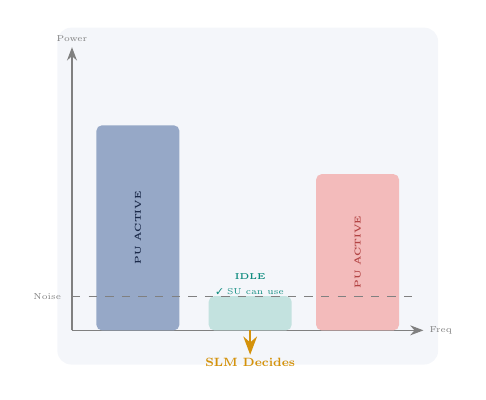
\begin{tikzpicture}[scale=0.62, transform shape]
  \fill[lightbg, rounded corners=5pt] (-0.3,-0.7) rectangle (7.5,6.2);
  \draw[-Stealth, gray] (0,0) -- (7.2,0) node[right,font=\tiny]{Freq};
  \draw[-Stealth, gray] (0,0) -- (0,5.8) node[above,font=\tiny]{Power};
  \fill[royalblue!50, rounded corners=2pt] (0.5,0) rectangle (2.2,4.2);
  \node[font=\tiny\bfseries, rotate=90, text=navy] at (1.35,2.1) {PU ACTIVE};
  \fill[teal!25, rounded corners=2pt] (2.8,0) rectangle (4.5,0.7);
  \node[font=\tiny\bfseries, text=teal] at (3.65,1.1) {IDLE};
  \node[font=\tiny, text=teal] at (3.65,0.8) {\cmark\ SU can use};
  \fill[coral!40, rounded corners=2pt] (5.0,0) rectangle (6.7,3.2);
  \node[font=\tiny\bfseries, rotate=90, text=coral!80!black] at (5.85,1.6) {PU ACTIVE};
  \draw[gray, dashed] (0,0.7) -- (7.1,0.7);
  \node[font=\tiny, text=gray, anchor=east] at (-0.1,0.7) {Noise};
  \draw[amber, thick, -Stealth] (3.65,0) -- (3.65,-0.5);
  \node[font=\scriptsize\bfseries, text=amber] at (3.65,-0.65) {SLM Decides};
\end{tikzpicture}
\end{center}
\end{column}
\end{columns}
\end{frame}


%##########################################################
\section{Dataset Overview}
%##########################################################
\begin{frame}{Dataset Overview --- Hardware \& Schema}
\small
\begin{columns}[T]
\begin{column}{0.48\textwidth}
\begin{block}{Hardware Setup}
\footnotesize
\renewcommand{\arraystretch}{1.2}
\begin{tabular}{@{}rl@{}}
\textbf{SDR Device}  & ADALM-Pluto \\
\textbf{Frequency}   & 2.4\,GHz (ISM) \\
\textbf{Sample Rate} & 1.024\,MHz \\
\textbf{Software}    & GNU Radio 3.10 \\
\textbf{FFT Size}    & 1024-point \\
\textbf{Modulations} & BPSK, QPSK, 8PSK, 16QAM \\
\end{tabular}
\end{block}
\end{column}

\begin{column}{0.48\textwidth}
\begin{block}{Data Schema (per row = one PSD snapshot)}
\footnotesize
\renewcommand{\arraystretch}{1.2}
\begin{tabular}{@{}ll@{}}
\texttt{Timestamp}     & Unix epoch time \\
\texttt{Mean\_PSD\_dB} & Power spectral density (dB) \\
\texttt{SNR\_dB}       & Signal-to-noise ratio (dB) \\
\texttt{PU\_Present}   & 0 or 1 (target label) \\
\texttt{Modulation}    & BPSK / QPSK / 8PSK / 16QAM \\
\end{tabular}
\end{block}
\end{column}
\end{columns}

\vspace{4pt}

\begin{columns}[T]
\begin{column}{0.48\textwidth}
\begin{block}{Dataset Sizes}
\footnotesize
\renewcommand{\arraystretch}{1.2}
\begin{tabular}{@{}lrl@{}}
\toprule
\textbf{Dataset} & \textbf{Rows} & \textbf{Use} \\
\midrule
Symbol Set 1 & 76{,}560 & Training \\
Symbol Set 2 & 44{,}824 & Validation \\
Symbol Set 3 & 31{,}594 & Testing \\
\midrule
\textbf{Total} & \textbf{152{,}978} & \\
\bottomrule
\end{tabular}
\end{block}
\end{column}

\begin{column}{0.48\textwidth}
\begin{exampleblock}{Full PSD Vectors (\texttt{.pth} files)}
\footnotesize
PyTorch tensors with \textbf{176-bin} full spectral shape per snapshot, binned by SNR = $[4, 6, \ldots, 20]$\,dB.

\smallskip
Each vector is a ``sentence'' of spectral tokens --- the \textbf{key input for the SLM}.
\end{exampleblock}
\end{column}
\end{columns}
\end{frame}


%##########################################################
\section{Exploratory Data Analysis}
%##########################################################
\begin{frame}{EDA --- Class Distribution}
\small
\begin{columns}[T]
\begin{column}{0.48\textwidth}
\begin{center}
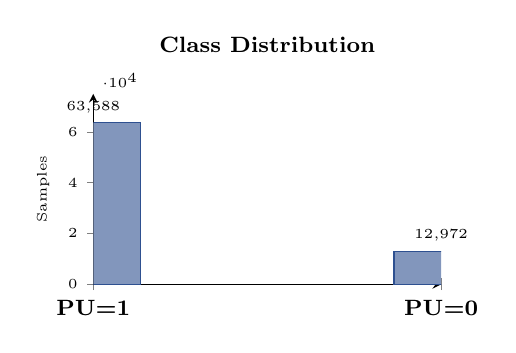
\begin{tikzpicture}
\begin{axis}[
    ybar, width=6cm, height=4cm,
    ylabel={\tiny Samples},
    symbolic x coords={PU=1, PU=0},
    xtick=data, xticklabel style={font=\footnotesize\bfseries},
    yticklabel style={font=\tiny},
    ymin=0, ymax=75000,
    bar width=1.2cm, enlarge x limits=0.5,
    nodes near coords, nodes near coords style={font=\tiny\bfseries},
    axis lines=left,
    title={\footnotesize\bfseries Class Distribution},
    title style={at={(0.5,1.08)}},
]
\addplot[fill=royalblue!60, draw=royalblue] coordinates {
    (PU=1, 63588) (PU=0, 12972)
};
\end{axis}
\end{tikzpicture}
\end{center}

\begin{alertblock}{Class Imbalance}
\footnotesize \textbf{83\% PU=1} vs.\ \textbf{17\% PU=0}. Needs focal loss, class weighting, or oversampling.
\end{alertblock}
\end{column}

\begin{column}{0.48\textwidth}
\begin{block}{Feature Statistics by PU Status}
\footnotesize
\renewcommand{\arraystretch}{1.2}
\begin{tabular}{@{}lcc@{}}
\toprule
 & \textbf{PU=1} & \textbf{PU=0} \\
\midrule
Mean PSD   & $-15.3$\,dB & $-21.1$\,dB \\
Mean SNR   & $10.6$\,dB  & $7.1$\,dB \\
SNR range  & 5--20\,dB   & 3--8\,dB \\
PSD range  & $-34$ to $+1$ & $-36$ to $+1$ \\
Count      & 63{,}588 & 12{,}972 \\
\bottomrule
\end{tabular}
\end{block}

\vspace{2pt}

\begin{exampleblock}{Key Insight}
\footnotesize
\textbf{SNR $<$ 8\,dB} is the hardest zone --- maximum class overlap. Higher-order modulations (8PSK, 16QAM) are harder to detect at low SNR.
\end{exampleblock}
\end{column}
\end{columns}
\end{frame}


%##########################################################
\section{Core Idea --- NLP Meets RF}
%##########################################################
\begin{frame}{The Big Idea --- NLP Meets Spectrum Sensing}
\small
\begin{center}
\renewcommand{\arraystretch}{1.4}
\begin{tabular}{@{} >{\bfseries\color{royalblue}}l c >{\bfseries\color{teal}}l @{}}
\toprule
\textbf{\color{navy}NLP World} & & \textbf{\color{navy}Spectrum World} \\
\midrule
Word / Token        & $\longleftrightarrow$ & Frequency bin PSD value \\
Sentence            & $\longleftrightarrow$ & Full PSD vector (176 bins) \\
Document            & $\longleftrightarrow$ & Temporal PSD sequence \\
Vocabulary (50K)    & $\longleftrightarrow$ & Quantized PSD levels (256) \\
Next Word Predict.  & $\longleftrightarrow$ & Next PSD prediction \\
Sentiment Analysis  & $\longleftrightarrow$ & PU detection (0 / 1) \\
Text Classification & $\longleftrightarrow$ & Modulation classification \\
\bottomrule
\end{tabular}
\end{center}

\vspace{6pt}

\begin{block}{}
\centering\small
\textbf{Core Insight:} Just as GPT reads sequences of \textcolor{royalblue}{\textbf{word tokens}} to understand language,\\
our SLM reads sequences of \textcolor{teal}{\textbf{spectral tokens}} to understand spectrum occupancy.
\end{block}
\end{frame}


%##########################################################
% WHY SLM > ML
%##########################################################
\begin{frame}{Why SLM Over Traditional ML?}
\small
\begin{center}
\renewcommand{\arraystretch}{1.35}
\begin{tabular}{@{}p{3cm} c c@{}}
\toprule
\textbf{Feature} &
\textbf{\textcolor{coral}{Traditional ML}} &
\textbf{\textcolor{teal}{Spectrum-SLM}} \\
\midrule
\rowcolor{lightbg}
Input features     & \xmark\ 2 features only     & \cmark\ 176-bin PSD \\
Temporal context   & \xmark\ Single snapshot      & \cmark\ Sequences \\
\rowcolor{lightbg}
Multi-task         & \xmark\ Separate models      & \cmark\ One model, 4 heads \\
Adaptability       & \xmark\ Retrain from scratch & \cmark\ Fine-tune \\
\rowcolor{lightbg}
Low SNR            & \xmark\ Degrades rapidly     & \cmark\ Subtle patterns \\
Generative         & \xmark\ Not possible         & \cmark\ Predicts future \\
\bottomrule
\end{tabular}
\end{center}

\vspace{4pt}

\begin{exampleblock}{Existing Baseline}
\footnotesize
A \textbf{VotingClassifier} (soft voting) with RandomForest (200 trees) + XGBoost (200 trees, lr=0.05) + AdaBoost (150 estimators), using only 2 features: Mean\_PSD\_dB and SNR\_dB.
\end{exampleblock}
\end{frame}


%##########################################################
\section{SLM Architecture}
%##########################################################
\begin{frame}{SLM Architecture}
\begin{center}
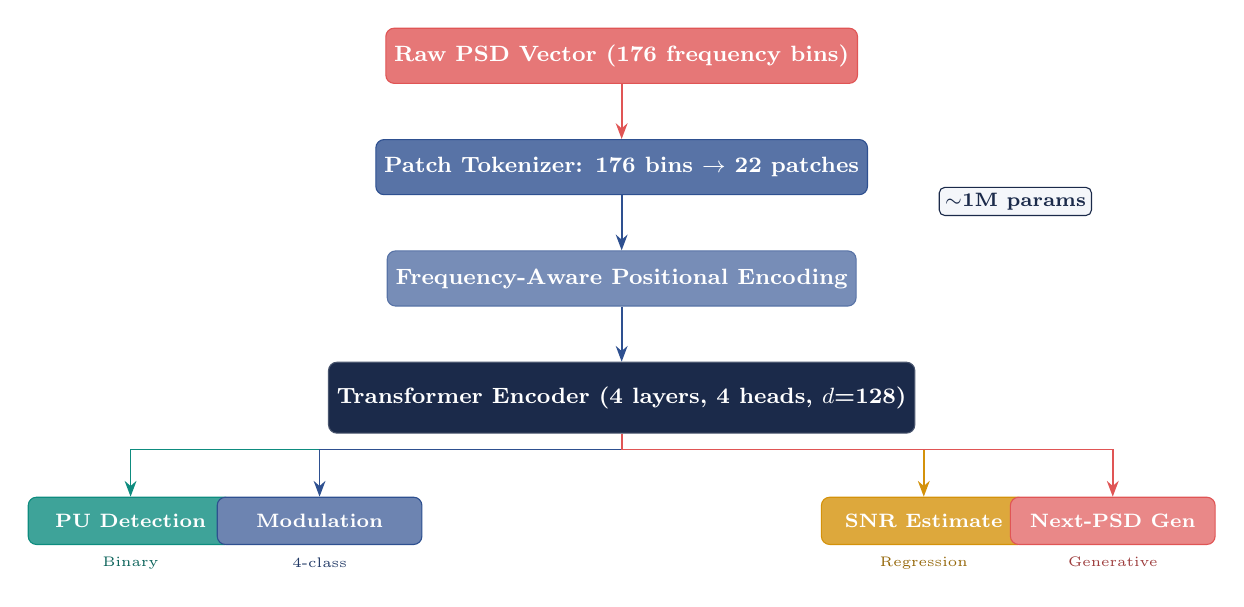
\begin{tikzpicture}[
  block/.style={rectangle, rounded corners=3pt, minimum width=4.5cm,
    minimum height=0.7cm, draw, font=\footnotesize\bfseries, text=white, inner sep=3pt},
  head/.style={rectangle, rounded corners=3pt, minimum width=2.6cm,
    minimum height=0.6cm, draw, font=\scriptsize\bfseries, inner sep=2pt},
  arr/.style={-Stealth, semithick},
  node distance=0.7cm,
]
  \node[block, fill=coral!80, draw=coral] (input) {Raw PSD Vector (176 frequency bins)};
  \node[block, fill=royalblue!80, draw=royalblue, below=of input] (token)
    {Patch Tokenizer: 176 bins $\to$ 22 patches};
  \node[block, fill=royalblue!65, draw=royalblue!80, below=of token] (pos)
    {Frequency-Aware Positional Encoding};
  \node[block, fill=navy, draw=navy!80, below=of pos, minimum height=0.9cm, minimum width=5.5cm] (trans)
    {Transformer Encoder (4 layers, 4 heads, $d$=128)};

  \node[head, fill=teal!80, draw=teal, text=white,
    below left=0.8cm and 1.2cm of trans] (h1) {PU Detection};
  \node[head, fill=royalblue!70, draw=royalblue, text=white,
    below left=0.8cm and -1.2cm of trans] (h2) {Modulation};
  \node[head, fill=amber!80, draw=amber, text=white,
    below right=0.8cm and -1.2cm of trans] (h3) {SNR Estimate};
  \node[head, fill=coral!70, draw=coral, text=white,
    below right=0.8cm and 1.2cm of trans] (h4) {Next-PSD Gen};

  \draw[arr, coral] (input) -- (token);
  \draw[arr, royalblue] (token) -- (pos);
  \draw[arr, royalblue] (pos) -- (trans);
  \draw[arr, teal] (trans.south) -- ++(0,-0.2) -| (h1.north);
  \draw[arr, royalblue] (trans.south) -- ++(0,-0.2) -| (h2.north);
  \draw[arr, amber] (trans.south) -- ++(0,-0.2) -| (h3.north);
  \draw[arr, coral] (trans.south) -- ++(0,-0.2) -| (h4.north);

  \node[font=\tiny, text=teal!70!black] at (h1.south) [below=1pt] {Binary};
  \node[font=\tiny, text=royalblue!70!black] at (h2.south) [below=1pt] {4-class};
  \node[font=\tiny, text=amber!70!black] at (h3.south) [below=1pt] {Regression};
  \node[font=\tiny, text=coral!70!black] at (h4.south) [below=1pt] {Generative};

  \node[font=\scriptsize\bfseries, text=navy, fill=lightbg, draw=navy,
    rounded corners=2pt, inner sep=2pt] at (5, -1.85) {$\sim$1M params};
\end{tikzpicture}
\end{center}
\end{frame}


%##########################################################
% MODEL SPECS
%##########################################################
\begin{frame}{Model Specifications}
\small
\begin{columns}[T]
\begin{column}{0.45\textwidth}
\begin{block}{Hyperparameters}
\footnotesize
\renewcommand{\arraystretch}{1.3}
\begin{tabular}{@{}ll@{}}
\toprule
\textbf{Parameter} & \textbf{Value} \\
\midrule
$d_\text{model}$     & 128 \\
$n_\text{heads}$     & 4 \\
$n_\text{layers}$    & 4--6 \\
$d_\text{ff}$        & 512 \\
Patch size            & 8 frequency bins \\
Num patches           & 22 \\
Dropout               & 0.1 \\
\textbf{Total params} & \textbf{$\sim$1M} \\
\bottomrule
\end{tabular}
\end{block}
\end{column}

\begin{column}{0.50\textwidth}
\begin{block}{Why ``Small'' Works}
\footnotesize
\begin{itemize}
  \item 176 bins $\ll$ 50K+ text vocabulary
  \item Spectral patterns simpler than language
  \item Only 4 modulation classes + binary detection
\end{itemize}
\end{block}

\vspace{2pt}

\begin{exampleblock}{Real-Time Feasibility}
\footnotesize
\begin{tabular}{@{}cl@{}}
  \cmark & Inference $< 10$\,ms \\
  \cmark & Runs on CPU \\
  \cmark & ONNX exportable \\
  \cmark & INT8 quantizable \\
\end{tabular}
\end{exampleblock}
\end{column}
\end{columns}
\end{frame}


%##########################################################
\section{Training Strategy}
%##########################################################
\begin{frame}{Training Strategy --- 3 Phases}
\begin{center}
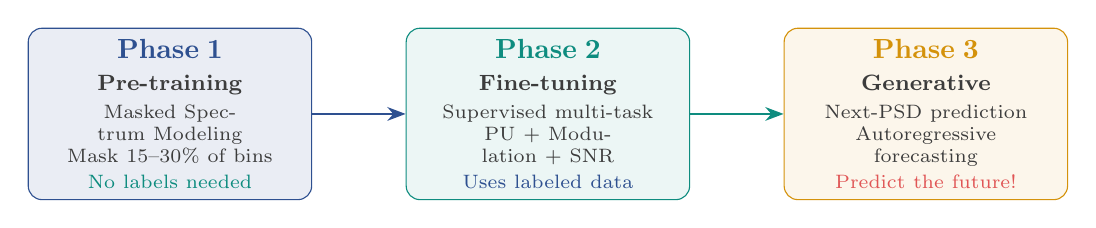
\begin{tikzpicture}[
  phase/.style={rectangle, rounded corners=5pt, draw, minimum width=3.6cm,
    minimum height=2cm, text width=3.2cm, align=center,
    font=\footnotesize, inner sep=4pt},
  arr/.style={-Stealth, thick},
]
  \node[phase, fill=royalblue!10, draw=royalblue, text=darkgray] (p1) at (0,0) {
    {\normalsize\bfseries\color{royalblue} Phase 1}\\[2pt]
    \textbf{Pre-training}\\[2pt]
    {\scriptsize Masked Spectrum Modeling\\
    Mask 15--30\% of bins\\
    \textcolor{teal}{No labels needed}}
  };
  \node[phase, fill=teal!8, draw=teal, text=darkgray] (p2) at (4.8,0) {
    {\normalsize\bfseries\color{teal} Phase 2}\\[2pt]
    \textbf{Fine-tuning}\\[2pt]
    {\scriptsize Supervised multi-task\\
    PU + Modulation + SNR\\
    \textcolor{royalblue}{Uses labeled data}}
  };
  \node[phase, fill=amber!8, draw=amber, text=darkgray] (p3) at (9.6,0) {
    {\normalsize\bfseries\color{amber} Phase 3}\\[2pt]
    \textbf{Generative}\\[2pt]
    {\scriptsize Next-PSD prediction\\
    Autoregressive forecasting\\
    \textcolor{coral}{Predict the future!}}
  };
  \draw[arr, royalblue] (p1.east) -- (p2.west);
  \draw[arr, teal] (p2.east) -- (p3.west);
\end{tikzpicture}
\end{center}

\vspace{4pt}

\small
\begin{columns}[T]
\begin{column}{0.30\textwidth}
\centering{\footnotesize\bfseries\color{royalblue} MSM Loss}\\[2pt]
$\displaystyle\mathcal{L}_\text{MSM}\!=\!\frac{1}{|\mathcal{M}|}\!\sum_{i \in \mathcal{M}}\!\|\hat{x}_i\!-\!x_i\|^2$
\end{column}
\begin{column}{0.35\textwidth}
\centering{\footnotesize\bfseries\color{teal} Multi-Task Loss}\\[2pt]
$\mathcal{L} = \alpha\mathcal{L}_\text{PU} + \beta\mathcal{L}_\text{mod} + \gamma\mathcal{L}_\text{SNR}$
\end{column}
\begin{column}{0.30\textwidth}
\centering{\footnotesize\bfseries\color{amber} Autoregressive}\\[2pt]
$P(\mathbf{x}_t \mid \mathbf{x}_{t\text{-}L:t\text{-}1})$
\end{column}
\end{columns}
\end{frame}


%##########################################################
\section{Implementation Roadmap}
%##########################################################
\begin{frame}{Implementation Roadmap}
\footnotesize
\begin{center}
\renewcommand{\arraystretch}{1.3}
\begin{tabular}{@{} c >{\bfseries\color{royalblue}}l p{8.5cm} @{}}
\toprule
\textbf{Step} & \textbf{Phase} & \textbf{Tasks} \\
\midrule
\rowcolor{lightbg}
\textcolor{white}{\textbf{\colorbox{royalblue}{1}}} &
Data Pipeline &
Load \texttt{.pth} files (176-bin PSD vectors) $\to$ normalize per-bin $\to$ create sliding-window sequences $\to$ stratified train/val/test split \\

\textcolor{white}{\textbf{\colorbox{teal}{2}}} &
\color{teal} Tokenization &
Patch-based embedding (8 bins $\to$ 22 patches per PSD) $\to$ add frequency-aware positional encoding $\to$ add temporal position encoding for sequences \\

\rowcolor{lightbg}
\textcolor{white}{\textbf{\colorbox{navy}{3}}} &
\color{navy} Model Training &
Phase 1: Masked Spectrum Modeling (self-supervised) $\to$ Phase 2: supervised multi-task fine-tuning $\to$ Phase 3: autoregressive generation \\

\textcolor{white}{\textbf{\colorbox{amber}{4}}} &
\color{amber!80!black} Evaluation &
Compare vs.\ VotingClassifier baseline $\to$ low-SNR ($<$8\,dB) analysis $\to$ latency benchmarks $\to$ ONNX export for deployment \\
\bottomrule
\end{tabular}
\end{center}

\vspace{4pt}
\begin{center}
\textcolor{royalblue}{\textbf{Step 1}} $\;\longrightarrow\;$
\textcolor{teal}{\textbf{Step 2}} $\;\longrightarrow\;$
\textcolor{navy}{\textbf{Step 3}} $\;\longrightarrow\;$
\textcolor{amber}{\textbf{Step 4}}
\end{center}
\end{frame}


%##########################################################
% TECH STACK & TIMELINE
%##########################################################
\begin{frame}{Tech Stack \& Timeline}
\small
\begin{columns}[T]
\begin{column}{0.45\textwidth}
\begin{block}{Tech Stack}
\footnotesize
\renewcommand{\arraystretch}{1.3}
\begin{tabular}{@{}ll@{}}
\textbf{Framework}  & PyTorch / Lightning \\
\textbf{Data}       & NumPy, Pandas, sklearn \\
\textbf{SDR}        & GNU Radio 3.10 \\
\textbf{Deploy}     & ONNX Runtime \\
\textbf{Hardware}   & ADALM-Pluto SDR \\
\end{tabular}
\end{block}
\end{column}

\begin{column}{0.50\textwidth}
\begin{exampleblock}{Estimated Timeline}
\footnotesize
\renewcommand{\arraystretch}{1.3}
\begin{tabular}{@{}ll@{}}
\toprule
\textbf{Period} & \textbf{Task} \\
\midrule
Week 1--2 & Data pipeline + tokenizer \\
Week 3--4 & Phase 1: pre-training (MSM) \\
Week 5--6 & Phase 2: supervised fine-tuning \\
Week 7--8 & Phase 3: generative + eval \\
\bottomrule
\end{tabular}
\end{exampleblock}
\end{column}
\end{columns}
\end{frame}


%##########################################################
\section{Expected Results}
%##########################################################
\begin{frame}{Expected Results --- Baseline vs.\ SLM}
\small
\begin{center}
\renewcommand{\arraystretch}{1.4}
\begin{tabular}{@{}p{4cm} >{\centering\arraybackslash}p{2cm}
  >{\centering\arraybackslash}p{2cm} p{4cm}@{}}
\toprule
\textbf{Task} &
\textbf{\textcolor{coral}{Baseline}} &
\textbf{\textcolor{teal}{SLM}} &
\textbf{Reason} \\
\midrule
\rowcolor{lightbg}
PU Detection (overall)  & 92--95\% & \textcolor{teal}{\textbf{96--98\%}} & Full PSD + attention \\
PU @ SNR$<$8\,dB        & 80--85\% & \textcolor{teal}{\textbf{90--94\%}} & Subtle spectral features \\
\rowcolor{lightbg}
Modulation Classif.     & 85--88\% & \textcolor{teal}{\textbf{92--95\%}} & Spectral signatures \\
SNR Estimation (MAE)    & N/A      & \textcolor{teal}{\textbf{$<$1.5\,dB}} & Regression head \\
\rowcolor{lightbg}
Inference Latency       & $\sim$1\,ms & \textbf{$<$10\,ms} & Still real-time \\
\bottomrule
\end{tabular}
\end{center}

\vspace{4pt}

\begin{block}{Key Takeaways}
\footnotesize
\begin{itemize}
  \item \textbf{8--12\% accuracy gain at low SNR} ($<$8\,dB) --- the hardest zone
  \item \textbf{Single model} handles all 4 tasks simultaneously
  \item \textbf{Generative capability} enables spectrum prediction --- impossible with traditional ML
\end{itemize}
\end{block}
\end{frame}


%##########################################################
\section{Risks \& Mitigations}
%##########################################################
\begin{frame}{Risks \& Mitigations}
\footnotesize
\renewcommand{\arraystretch}{1.35}
\begin{center}
\begin{tabular}{@{}
  p{3cm}
  >{\centering\arraybackslash}p{1.3cm}
  p{7.5cm}@{}}
\toprule
\textbf{\textcolor{coral}{Risk}} & \textbf{Impact} & \textbf{\textcolor{teal}{Mitigation}} \\
\midrule
\rowcolor{lightbg}
Small dataset ($\sim$150K) &
\textcolor{amber}{\textbf{Med}} &
Data augmentation: noise injection, spectral shifting, mixup \\

Class imbalance (83/17) &
\textcolor{coral}{\textbf{High}} &
Focal loss ($\gamma\!=\!2$), class weighting, SMOTE oversampling \\

\rowcolor{lightbg}
Real-time latency &
\textcolor{amber}{\textbf{Med}} &
Patch tokenization (22 vs 176 tokens), INT8 quantization \\

Overfitting &
\textcolor{coral}{\textbf{High}} &
Dropout, early stopping, cross-validation across symbol sets \\

\rowcolor{lightbg}
Edge deployment &
\textcolor{amber}{\textbf{Med}} &
Knowledge distillation, ONNX export, model compression \\
\bottomrule
\end{tabular}
\end{center}
\end{frame}


%##########################################################
\section{Research Novelty}
%##########################################################
\begin{frame}{Research Novelty}
\small
\begin{columns}[T]
\begin{column}{0.52\textwidth}
\begin{block}{5 Novel Contributions}
\footnotesize
\begin{enumerate}
  \item \textbf{First SLM for Spectrum Sensing}\\
    {\scriptsize No prior GPT-style modeling on PSD data}
  \item \textbf{Masked Spectrum Modeling}\\
    {\scriptsize Novel self-supervised pre-training for RF}
  \item \textbf{Multi-Task Intelligence}\\
    {\scriptsize Detection + Classification + Estimation}
  \item \textbf{Generative Spectrum Prediction}\\
    {\scriptsize Autoregressive PSD forecasting}
  \item \textbf{Real Hardware Data}\\
    {\scriptsize ADALM-Pluto SDR, not simulations}
\end{enumerate}
\end{block}
\end{column}

\begin{column}{0.44\textwidth}
\begin{exampleblock}{Target Venues}
\footnotesize
\begin{itemize}
  \item \textbf{IEEE TCCN}\\[-2pt]
    {\scriptsize Cognitive Comm.\ \& Networking}
  \item \textbf{IEEE DySPAN}\\[-2pt]
    {\scriptsize Dynamic Spectrum Access}
  \item \textbf{IEEE GLOBECOM / ICC}\\[-2pt]
    {\scriptsize Communications conferences}
  \item \textbf{IEEE WCL}\\[-2pt]
    {\scriptsize Wireless Comm.\ Letters}
\end{itemize}
\end{exampleblock}
\end{column}
\end{columns}
\end{frame}


%##########################################################
% THANK YOU
%##########################################################
{
\setbeamertemplate{footline}{}
\begin{frame}[plain]
\vfill
\begin{center}
  {\Huge\bfseries\color{navy} Thank You!}\\[10pt]
  {\Large\color{royalblue} Questions \& Discussion}\\[12pt]
  \textcolor{royalblue}{\rule{7cm}{1pt}}\\[12pt]
  {\normalsize
    \textbf{Anjani} \;\;$\bullet$\;\;
    \textbf{Ashish Joshi} \;\;$\bullet$\;\;
    \textbf{Mayank}}\\[6pt]
  {\small Guide: \textbf{Dr.\ Abhinandan S.P.}}\\[12pt]
  {\small\color{gray}
    152{,}978 samples \;\textbar\;
    $\sim$1M params \;\textbar\;
    Real SDR data \;\textbar\;
    Multi-task transformer}
\end{center}
\vfill
\end{frame}
}

\end{document}
